\section{Testing finale}

\begin{frame}{Testing finale}
    Abbiamo scelto di effettuare a seguito del refactoring gli stessi test effettuati sulla versione 5, in modo da verificare che le funzionalità corrette dell'applicazione rimanessero tali anche dopo il refactoring.\\\bigskip

    In particolare, i casi di test per la verifica dei requisiti e delle funzionalità sono stati scelti basandosi in modo più rigoroso rispetto al testing iniziale sulle linee guida che suggeriscono di effettuare test su:
    \begin{itemize}
        \item Classi di equivalenza
        \item Casi limite
    \end{itemize}
\end{frame}

%%%%%%%%%%%%%%%%%%%%%%%%%%%%%%%%%%%%%%%%%%
%          TEST CLASSE CATEGORY          %
%%%%%%%%%%%%%%%%%%%%%%%%%%%%%%%%%%%%%%%%%%

\begin{frame}{Test Classe Category}
    \framesubtitle{Test di classe}
    
    \begin{figure}
        \centering
        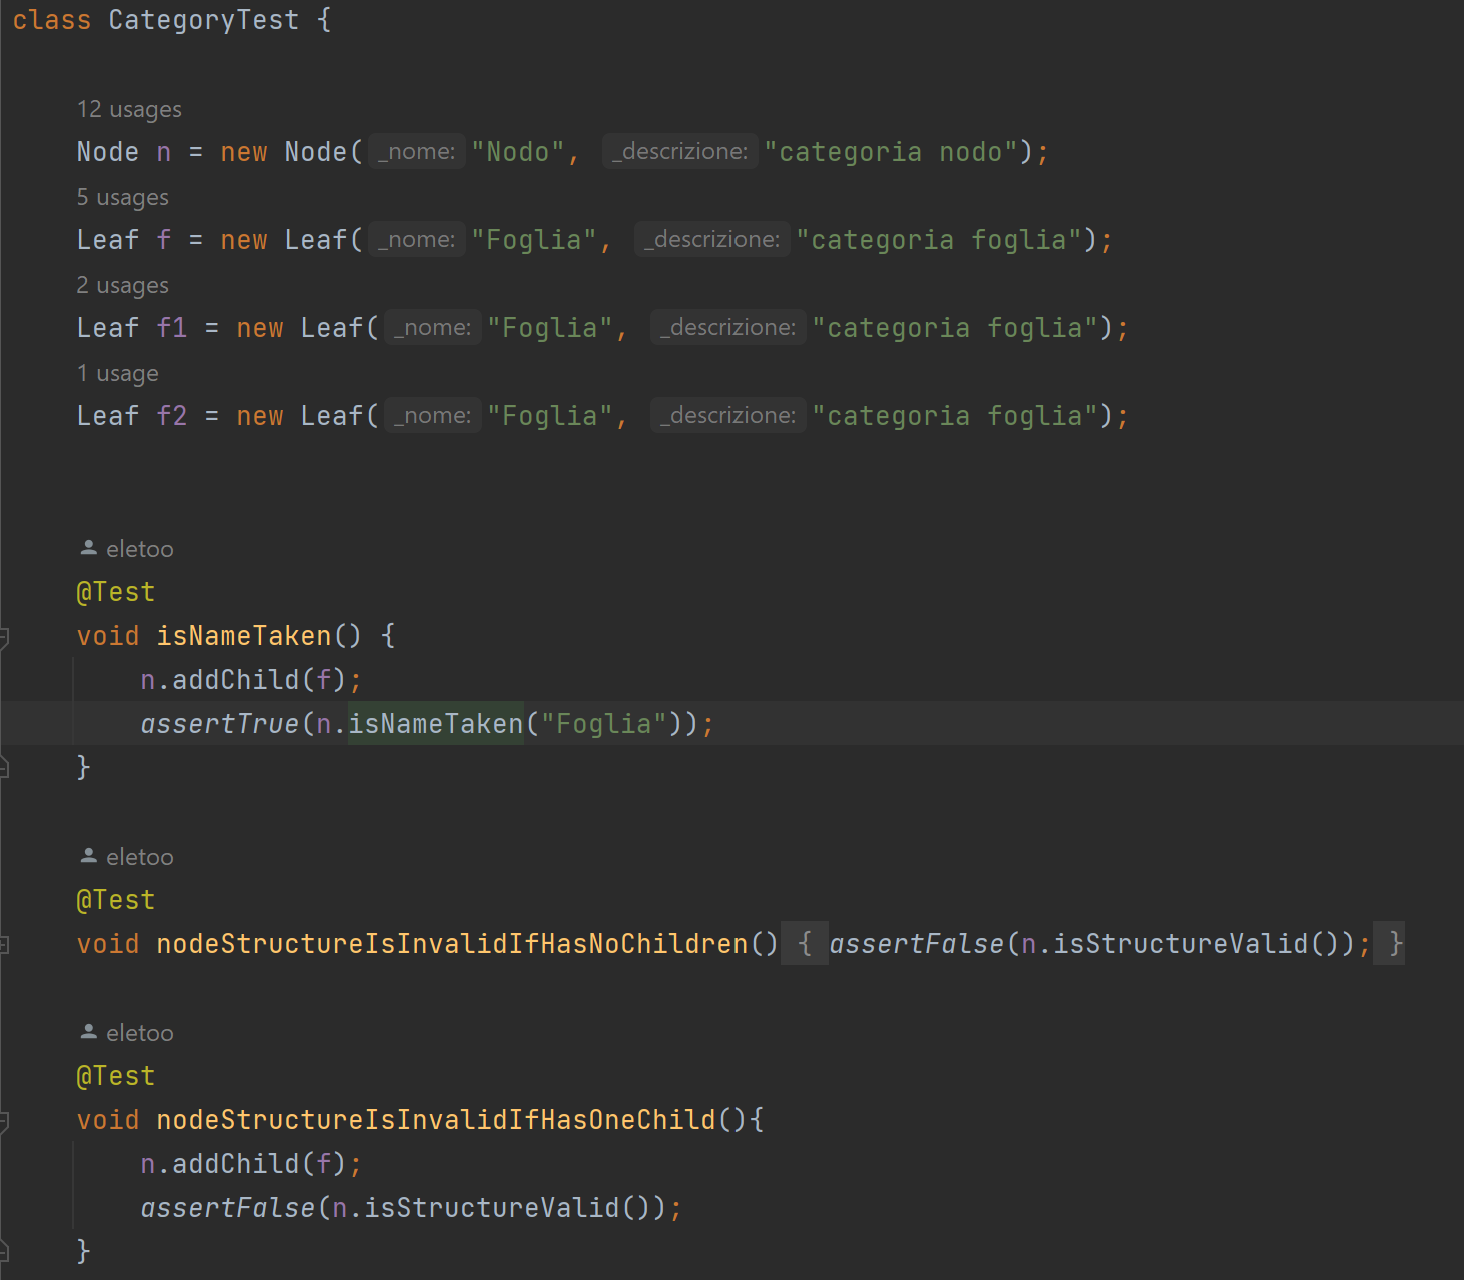
\includegraphics[width=.55\textwidth]{final testing/finaltesting-category1.png}
    \end{figure}    

    \note{
        Il test sulla classe \texttt{Categoria} non necessitava di subire particolari variazioni dal momento che gli unici cambiamenti apportati al codice che influissero sui test sono stati relativi ai nomi della classe \texttt{Categoria} in \texttt{Category}, \texttt{Foglia} in \texttt{Leaf} e \texttt{Nodo} in \texttt{Node}.
    }
\end{frame}

\begin{frame}{Test Classe Category}
    \begin{figure}
        \centering
        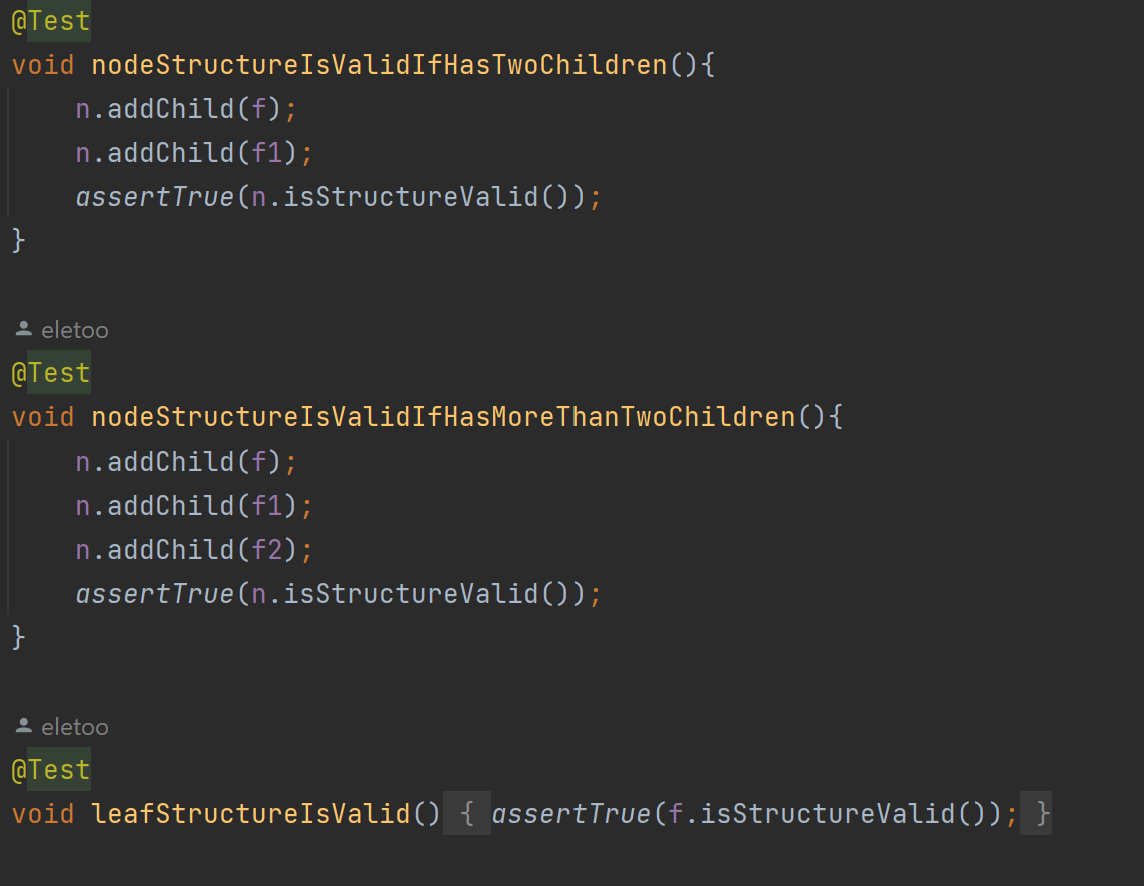
\includegraphics[width=.65\textwidth]{final testing/finaltesting-category2.png}
    \end{figure}
\end{frame}

%%%%%%%%%%%%%%%%%%%%%%%%%%%%%%%%%%%%%%%%%%
%          TEST CLASSE TIME              %
%%%%%%%%%%%%%%%%%%%%%%%%%%%%%%%%%%%%%%%%%%
\begin{frame}{Test Classe Time}
    \framesubtitle{Test di requisiti e funzionalità}
    
    \begin{figure}
        \centering
        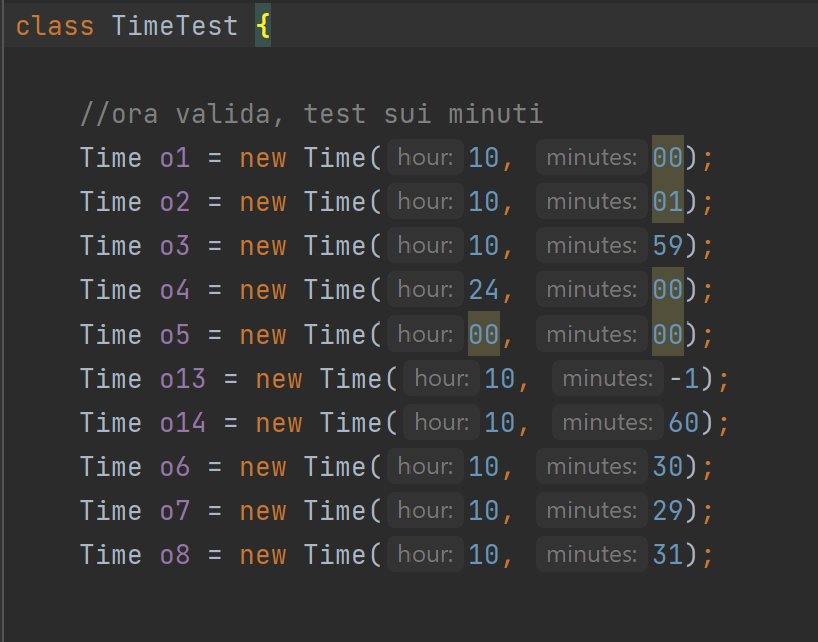
\includegraphics[width=.65\textwidth]{final testing/finaltesting-time1.png}
    \end{figure}    

    \note{
        Per il test delle funzionalità abbiamo mantenuto la scelta della funzionalità individuata per il testing iniziale:\\
        ``Gli orari per effettuare lo scambio possono essere solo allo scoccare dell'ora o alla mezza (ogni trenta minuti)''\\\bigskip
        La logica applicata per individuare i casi di test è quella delle classi di equivalenza e dei casi limite.\\
        Nella slide a fianco sono mostrati i casi di test individuati considerando orario valido e minuti invalidi.
    }

\end{frame}

\begin{frame}{Test Classe Time}
    
    \begin{figure}
        \centering
        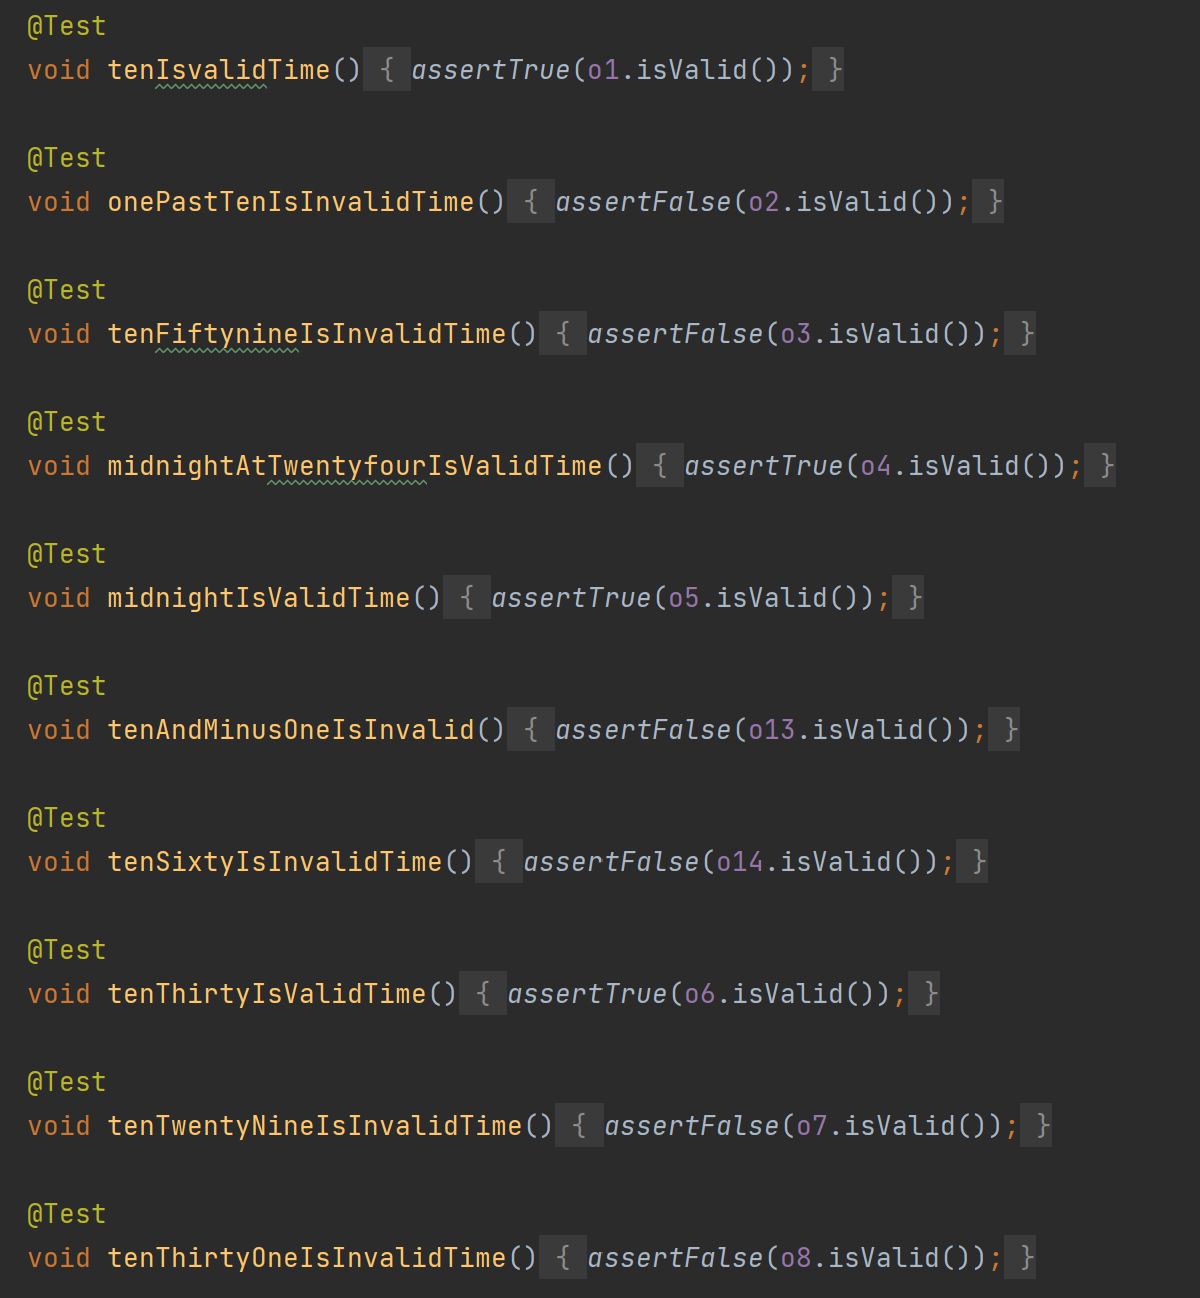
\includegraphics[width=.45\textwidth]{final testing/finaltesting-time2.png}
    \end{figure}    

    \note{
      Nella slide a fianco sono mostrati i metodi che testano i casi individuati considerando orario valido e minuti invalidi.
    }

\end{frame}

\begin{frame}{Test Classe Time}
    \framesubtitle{Test di requisiti e funzionalità}
    
    \begin{figure}
        \centering
        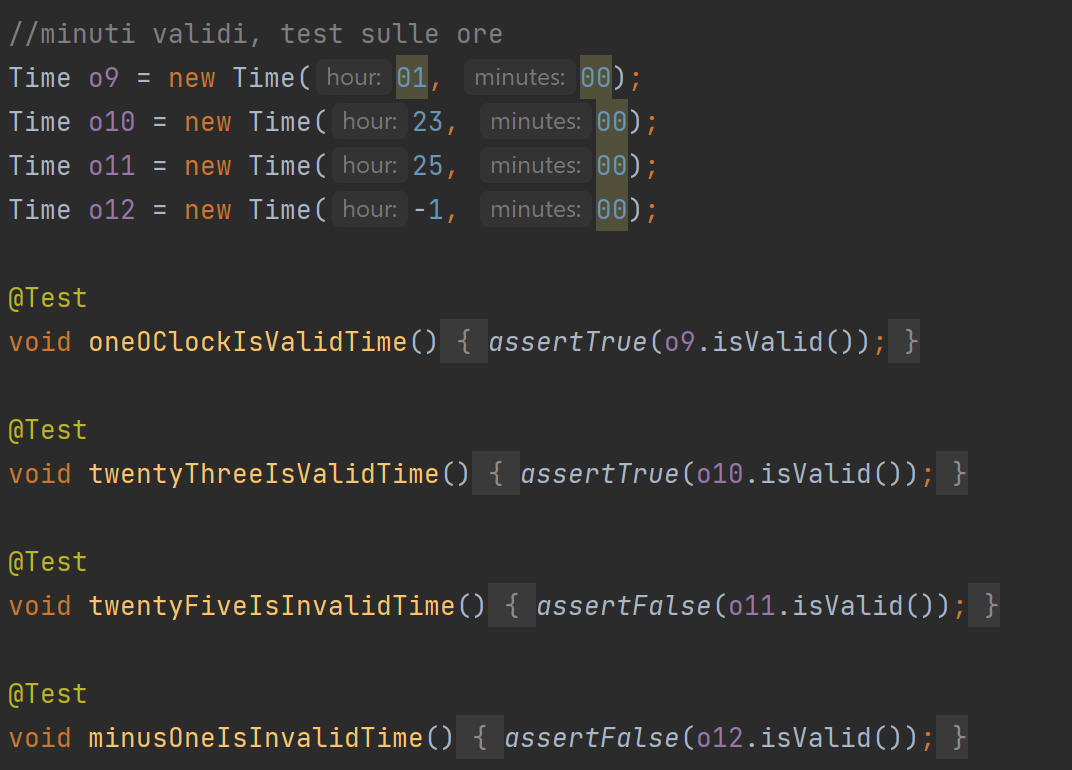
\includegraphics[width=.65\textwidth]{final testing/finaltesting-time3.png}
    \end{figure}    

    \note{
       Nella slide a fianco sono mostrati i casi di test individuati considerando orario invalido e minuti validi.
    }

\end{frame}